\documentclass[nobib]{tufte-handout}

\usepackage{amssymb}
\usepackage{hyperref}
\usepackage{pgfplots}
\usepackage[activate={true,nocompatibility},final,tracking=true,kerning=true,spacing=true,factor=1100,stretch=10,shrink=10]{microtype}
\usepackage{color}
\usepackage{steinmetz}
\usepackage{placeins}
\usepackage{marginfix}
\usepackage{array}
\usepackage{tikz}
\usepackage{amsmath}
\usepackage{amsthm}
\usepackage{booktabs}
\usepackage{listings}
\usepackage[edges]{forest}
\usepackage{caption}
\usepackage[T1]{fontenc}
\usepackage{lmodern}
\usepackage{units}
\usepackage{fancyvrb}
\usepackage{multicol}
\DeclareCaptionFont{white}{\color{white}}
\DeclareCaptionFormat{listing}{\colorbox{gray}{\parbox{\textwidth}{#1#2#3}}}
\captionsetup[lstlisting]{format=listing,labelfont=white,textfont=white}

% Set up the images/graphics package
\usepackage{graphicx}
\setkeys{Gin}{width=\linewidth,totalheight=\textheight,keepaspectratio}
\graphicspath{{.}}

\title{Notes for ECE 46300 - Introduction To Computer Communication Networks }
\author{Zeke Ulrich}
\date{\today} 

\fvset{fontsize=\normalsize}
\usetikzlibrary{shapes}
\usetikzlibrary{positioning}

% For finite state machines 
\usetikzlibrary{automata} % Import library for drawing automata
\usetikzlibrary{positioning} % ...positioning nodes
\usetikzlibrary{arrows} % ...customizing arrows
\tikzset{node distance=2.5cm, % Minimum distance between two nodes. Change if necessary.
    every state/.style={ % Sets the properties for each state
    semithick,
    fill=gray!10},
    initial text={}, % No label on start arrow
    double distance=2pt, % Adjust appearance of accept states
    every edge/.style={ % Sets the properties for each transition
    draw,
    ->,>=stealth', % Makes edges directed with bold arrowheads
    auto,
    semithick}}
\let\epsilon\varepsilon

% These commands are used to pretty-print LaTeX commands
\newcommand{\doccmd}[1]{\texttt{\textbackslash#1}}% command name -- adds backslash automatically
\newcommand{\docopt}[1]{\ensuremath{\langle}\textrm{\textit{#1}}\ensuremath{\rangle}}% optional command argument
\newcommand{\docarg}[1]{\textrm{\textit{#1}}}% (required) command argument
\newenvironment{docspec}{\begin{quote}\noindent}{\end{quote}}% command specification environment
\newcommand{\docenv}[1]{\textsf{#1}}% environment name
\newcommand{\docpkg}[1]{\texttt{#1}}% package name
\newcommand{\doccls}[1]{\texttt{#1}}% document class name
\newcommand{\docclsopt}[1]{\texttt{#1}}% document class option name

% Define a custom command for definitions and biconditional
\newcommand{\defn}[2]{\noindent\textbf{#1}:\ #2}
\let\biconditional\leftrightarrow

\begin{document}

\maketitle

\tableofcontents

\section{Course Description}
An introduction to the design and implementation of computer communication networks. The focus is on the concepts and the fundamental design principles that have contributed to the global Internet success. Topics include: digital transmission and multiplexing, protocols, MAC layer design (Ethernet/802.11), LAN interconnects and switching, congestion/flow/error control, routing, addressing, performance evaluation, internetworking (Internet) including TCP/IP, HTTP, DNS etc. This course will include one or more programming projects.
\pagebreak

\section{Computer Networks}

The high-level question this course will answer is "how do computers reliably
communicate?"

The answer is through computer networks, a group
of interconnected nodes or computing devices that
exchange data and resources with each other.

\begin{figure}[htbp]
    \centering
    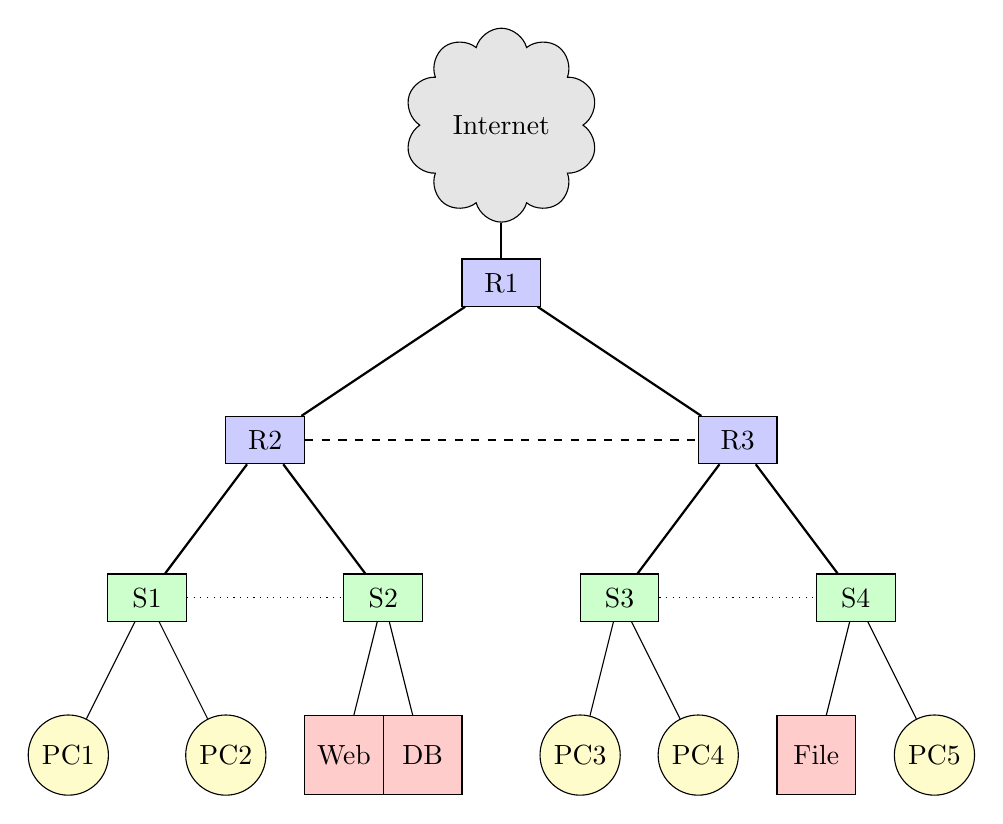
\begin{tikzpicture}[
            node distance=2cm,
            router/.style={rectangle, draw, fill=blue!20, minimum width=1cm, minimum height=0.6cm},
            switch/.style={rectangle, draw, fill=green!20, minimum width=1cm, minimum height=0.6cm},
            computer/.style={circle, draw, fill=yellow!20, minimum size=0.8cm},
            server/.style={rectangle, draw, fill=red!20, minimum width=1cm, minimum height=1cm},
            internet/.style={cloud, draw, fill=gray!20, minimum width=2cm, minimum height=1cm}
        ]

        % Internet cloud
        \node[internet] (internet) at (0,4) {Internet};

        % Core router
        \node[router] (core) at (0,2) {R1};

        % Distribution layer
        \node[router] (r2) at (-3,0) {R2};
        \node[router] (r3) at (3,0) {R3};

        % Access layer switches
        \node[switch] (s1) at (-4.5,-2) {S1};
        \node[switch] (s2) at (-1.5,-2) {S2};
        \node[switch] (s3) at (1.5,-2) {S3};
        \node[switch] (s4) at (4.5,-2) {S4};

        % End devices
        \node[computer] (pc1) at (-5.5,-4) {PC1};
        \node[computer] (pc2) at (-3.5,-4) {PC2};
        \node[server] (srv1) at (-2,-4) {Web};
        \node[server] (srv2) at (-1,-4) {DB};
        \node[computer] (pc3) at (1,-4) {PC3};
        \node[computer] (pc4) at (2.5,-4) {PC4};
        \node[server] (srv3) at (4,-4) {File};
        \node[computer] (pc5) at (5.5,-4) {PC5};

        % Connections
        % Internet to core
        \draw[thick] (internet) -- (core);

        % Core to distribution
        \draw[thick] (core) -- (r2);
        \draw[thick] (core) -- (r3);

        % Distribution to access
        \draw[thick] (r2) -- (s1);
        \draw[thick] (r2) -- (s2);
        \draw[thick] (r3) -- (s3);
        \draw[thick] (r3) -- (s4);

        % Redundant connections between distribution routers
        \draw[thick, dashed] (r2) -- (r3);

        % Access to end devices
        \draw (s1) -- (pc1);
        \draw (s1) -- (pc2);
        \draw (s2) -- (srv1);
        \draw (s2) -- (srv2);
        \draw (s3) -- (pc3);
        \draw (s3) -- (pc4);
        \draw (s4) -- (srv3);
        \draw (s4) -- (pc5);

        % Some cross-connections for redundancy
        \draw[dotted] (s1) -- (s2);
        \draw[dotted] (s3) -- (s4);

    \end{tikzpicture}
    \caption{Computer Network}
    \label{fig:computer-network}
\end{figure}

A computer network enables communication between users and their devices.

\begin{figure}[htbp]
    \centering
    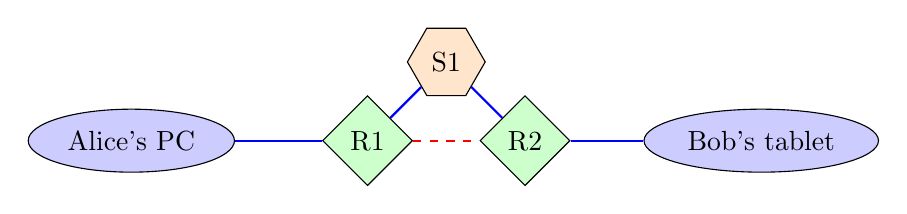
\begin{tikzpicture}[
            node distance=2.5cm,
            user/.style={ellipse, draw, fill=blue!20, minimum width=1.5cm, minimum height=0.8cm},
            device/.style={rectangle, draw, fill=yellow!20, minimum width=1cm, minimum height=0.6cm},
            router/.style={diamond, draw, fill=green!20, minimum width=1cm, minimum height=1cm},
            switch/.style={regular polygon, regular polygon sides=6, draw, fill=orange!20, minimum size=0.8cm}
        ]

        \node[user] (alice) at (-4,0) {Alice's PC};

        \node[user] (bob) at (4,0) {Bob's tablet};

        % Intermediate nodes
        \node[router] (r1) at (-1,0) {R1};
        \node[switch] (s1) at (0,1) {S1};
        \node[router] (r2) at (1,0) {R2};

        % Network path between Alice and Bob
        \draw[thick, blue] (alice) -- (r1);
        \draw[thick, blue] (r1) -- (s1);
        \draw[thick, blue] (s1) -- (r2);
        \draw[thick, blue] (r2) -- (bob);

        % Alternative path (dashed)
        \draw[thick, dashed, red] (r1) -- (r2);

    \end{tikzpicture}
    \caption{Simple Network}
    \label{fig:simple-network}
\end{figure}

The first stop that most home devices take in connecting to other
devices is the router. From there, the router can route data and
find a path for Alice's PC to get to Bob's tablet. The core of any
network is routers, which figure out the best way to get data from
one device to another device.

This process can get complex, with cell tower connections, different ISPs,
different edge devices, and more. Let's abstract the important elements
of the network.

\begin{itemize}
    \item Links: carry data from one endpoint to another
    \item End hosts: sitting at the edge of a network. Generate and receive data.
    \item Routers: forward data through the network.
\end{itemize}

Any network can be abstracted as a connection of links, end hosts, and routers.
We can thus represent any computer network as a graph, in the mathematical
sense, and apply all our graph algorithms to it.

A communication link can either be \emph{full} or \emph{half} duplex.
In a half duplex, a link can carry data in only one direction at a time.
In a full duplex, data transmission is bidirectional.
\marginnote{In this class, all links are assumed to be full duplex
    unless otherwise stated. }
If a link bandwidth is $B$, then a full-duplex link can carry $B$
in both directions simultaneously.
\section{Routing and Packets}

In our abstraction of routers, we leave the problem of finding
a path from end hosts unanswered. Since we can represent a computer
network as a graph, a shortest-path algorithm like Dijkstra's is a
relatively simple way to find a good path between Alice and Bob.
\section{Internet Architecture}

We need to solve these problems:
\begin{itemize}
    \item Name and addressing: identifiers for network nodes
    \item Destination discovery: finding the destination address
    \item Forwarding: sending received data to the next hop (neighbor)
    \item Routing: finding the path from source to destination
    \item Reliability: handling failures, packet drops, packet corruption
    \item Application multiplexing: delivering data from multiple host
          applications to the network and vice versa
\end{itemize}

\subsection{Name and Addressing}
Name is the human-readable name for each node (e.g., URL www.google.com).
Address is where node is located (e.g., IP address 172.21.4.110).

\subsection{Destination discovery}
When you go to a web page, you type the name in your browser. You
need to get the address still. The way names are resolved into
addresses is via the Domain Name System (DNS), a set of global
servers that maintain the mappings between host names and addresses.
When you type a URL, the browser contacts a DNS server to get the address.

\subsection{Forwarding}
A router has many ports. Each port in a router acts as both input
and output, i.e., you can both send and receive packets on each port
simultaneously.
When a packet arrives at a router, the router looks at the destination address
in the header. Based on destination address, the router consults the routing
table, determines the right output port, and sends the packet to that port's queue.
For each output port in parallel, when the port is free, the router picks
a packet from the corresponding output queue in some order (e.g. FIFO) and
sends the packet over the output port.

\subsection{Routing}
How do a network of routers collectively find a path between each
source and destination host? The answer is a routing protocol,
a distributed algorithm that runs independently at each router.
\section{Sockets}

A \emph{socket} is an OS mechanism for inter-process communication.
It allows two processes or applications on the same (loopback) or
different machines to communicate with each other. The communication path
goes through the network stack of machines running the processes.

The socket interface sits between the application and transport layer.
It has send and recieve buffers for each app, which apps access via
\texttt{send()} and \texttt{recieve()}. Each application is attached to
a socket that has a unique port number and send-recieve buffers.

\subsection{Connection}

A \emph{connection} is identified with a 5-tuple:
\begin{itemize}
    \item Local IP address
    \item Remote IP address
    \item Local port
    \item Remote port
    \item Transport protocol type
\end{itemize}
These 5 things in combination make a connection. A local and
remote socket make a connection.
\marginnote{Any address that begins with \texttt{127.} is
    on the local machine, i.e. on loopback.}

Creating a socket is the first step in socket programming.
Use the \texttt{socket()} system call, which returns a file
descriptor. This is interesting, because it abstracts the difficulties
of sending data over a network to the same process as writing
to a file.

There are three things needed to open a socket, which is done with a
call like \texttt{int fd = socket(int family, int type, int protocol)}
\begin{itemize}
    \item \texttt{family}: protocol family used for communication. E.g. \texttt{AF\_INET}.
    \item \texttt{type}: defines the communications semantics used. There are two
          popular choices, \texttt{SOCK\_STREAM} which is reliable, and \texttt{SOCK\_DGRAM}
          which is unreliable.
    \item \texttt{protocol}: specifies a particular transport protocol. Setting to 0
          will choose the default protocol implemented in the OS. E.g. TCP, UDP.
\end{itemize}

SOCK\_DGRAM is connectionless, i.e. no handshake required before sending data.
This is a packet or \emph{datagram} abstraction. SOCK\_DGRAM offers unreliable
communication in the sense that there is no promise that every packet is
delivered.

SOCK\_STREAM is connection-oriented, i.e. explicit handshake happens before
data is sent. This is a byte stream abstraction. SOCK\_STREAM offers reliable
communication, which means that all the data reaches its destination reliably and
in-order.

A recap of important function calls:

\begin{itemize}
    \item \texttt{socket()}: creates a socket
    \item \texttt{bind()}: bind socket to an address <IP, port>
    \item \texttt{connect()}: initiate connection to server
    \item \texttt{listen()}: listen for and queue incoming client connections
    \item \texttt{accept()}: accept incoming client connections
    \item \texttt{send()}: send data over a connected socket (TCP)
    \item \texttt{recv()}: receive data from a connected socket (TCP)
    \item \texttt{sendto()}: send data to a specific address (UDP)
    \item \texttt{recvfrom()}: receive data and sender's address (UDP)
    \item \texttt{close()}: close the socket and release resources
\end{itemize}
\section{Network Performance Metrics}

When evaluating if a network is good or bad, there are two key metrics:
\emph{bandwidth} or \emph{throughput} and \emph{delay} or \emph{latency}.
A good network should have high bandwidth/throughput and low delay.

\subsection{Bandwidth and Throughput}
Bandwidth is the max number of bits that can sent through a network
per unit time, typically measured in bits per second (bps).
Bandwidth is a property of the physical network components. For instance,
a copper cable may have a bandwidth of 500 Mbps or a fiber optic cable
may have a bandwidth of 100 Gbps.


Throughput measures the bandwidth utilization of a network. It's also
measured in bits per second.
\begin{equation}
    0 \leq \text{throughput} \leq \text{bandwidth}
\end{equation}
Throughput is a function of the mechanisms used to communicate over the
physical network. Network throughput can be lower than network bandwidth
due to inefficiencies of communication mechanism, but a good network
will make throughput as high as possible.

\subsection{Latency}
Suppose you are sending a series of bits from point A to B. Delay or
latency is the total time between first bit leaving point A and last
bit reaching point B. It is measured in units of time, typically seconds
or milliseconds.
\marginnote{Internet for outer space is currently an area of research.
    Latency can be minutes, hours, or days in such a case. }
Note that, in a packet-switched network, the entire packet must be
received by the router. This "store-and-forward" model introduces
delays. An alternative with smaller delay is "cut-through", where
the router begins processing as soon as the destination address is
received. The tradeoff is that routers can't check for packet
corruption, since it necessarily requires the entire packet.

We represent delays with a timing diagram, as in Figure \ref{fig:timingdiagram}.

\begin{figure}
    \centering
    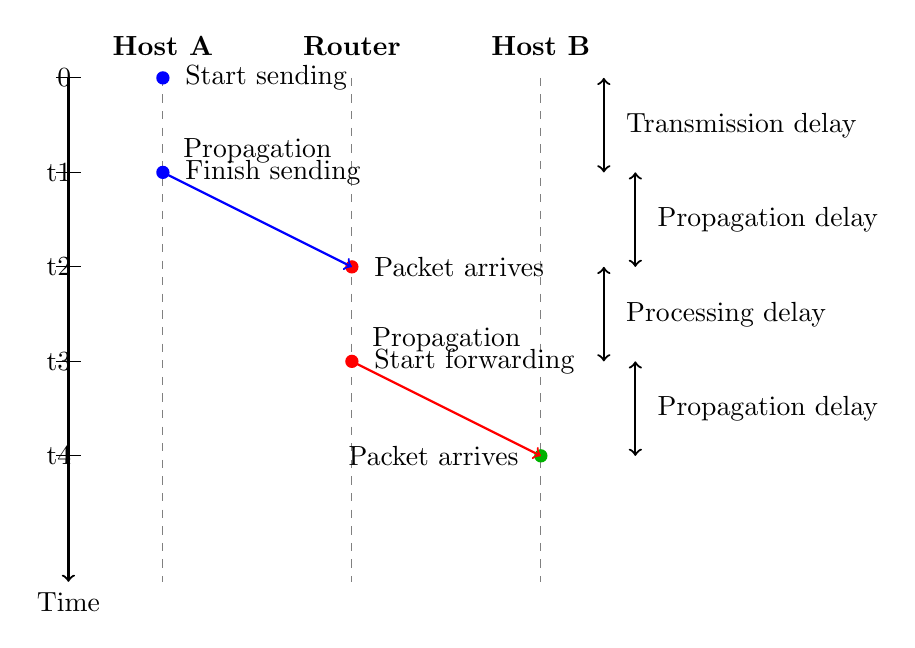
\begin{tikzpicture}[scale=0.8]
        % Time axis (vertical, going down)
        \draw[thick, ->] (-0.5, 0) -- (-0.5, -8) node[below] {Time};

        % Time labels
        \foreach \y/\label in {0/0, -1.5/t1, -3/t2, -4.5/t3, -6/t4} {
                \draw (-0.7, \y) -- (-0.3, \y) node[left] {\label};
            }

        % Host A, Router, Host B columns
        \node at (1, 0.5) {\textbf{Host A}};
        \node at (4, 0.5) {\textbf{Router}};
        \node at (7, 0.5) {\textbf{Host B}};

        % Vertical lines for each node
        \draw[dashed, gray] (1, 0) -- (1, -8);
        \draw[dashed, gray] (4, 0) -- (4, -8);
        \draw[dashed, gray] (7, 0) -- (7, -8);

        % Packet transmission events
        % Host A starts sending at t=0
        \fill[blue] (1, 0) circle (3pt);
        \node[right] at (1.2, 0) {Start sending};

        % Host A finishes sending at t₁
        \fill[blue] (1, -1.5) circle (3pt);
        \node[right] at (1.2, -1.5) {Finish sending};

        % Packet arrives at router at t₂
        \fill[red] (4, -3) circle (3pt);
        \node[right] at (4.2, -3) {Packet arrives};

        % Router starts forwarding at t₃
        \fill[red] (4, -4.5) circle (3pt);
        \node[right] at (4.2, -4.5) {Start forwarding};

        % Packet arrives at Host B at t₄
        \fill[green!70!black] (7, -6) circle (3pt);
        \node[left] at (6.8, -6) {Packet arrives};

        % Arrows showing packet flow
        \draw[->, thick, blue] (1, -1.5) -- (4, -3);
        \node[above, sloped] at (2.5, -1.5) {Propagation};

        \draw[->, thick, red] (4, -4.5) -- (7, -6);
        \node[above, sloped] at (5.5, -4.5) {Propagation};

        % Delay annotations
        \draw[<->, thick] (8, 0) -- (8, -1.5);
        \node[right] at (8.2, -0.75) {Transmission delay};

        \draw[<->, thick] (8.5, -1.5) -- (8.5, -3);
        \node[right] at (8.7, -2.25) {Propagation delay};

        \draw[<->, thick] (8, -3) -- (8, -4.5);
        \node[right] at (8.2, -3.75) {Processing delay};

        \draw[<->, thick] (8.5, -4.5) -- (8.5, -6);
        \node[right] at (8.7, -5.25) {Propagation delay};

    \end{tikzpicture}
    \caption{Timing Diagram}
    \label{fig:timingdiagram}
\end{figure}

There are different delays when packet routing:
\begin{itemize}
    \item Transmission Delay: Packet Size / Link Bandwidth
    \item Propagation Delay: Link Length / Link Propagation Speed
    \item Queuing Delay: Sum of Transmission Delay for all packets
          ahead in the queue
    \item Processing Delay: Depends upon the router hardware
          processing speed, nature of processing, etc.
\end{itemize}

The total delay for a single packet going over 2 hops in a
store-and-forward packet-switched network is
\begin{equation}
    2(TD + PD) + QD + PrD
\end{equation}

For $M$ hops ($M-1$ routers) the end-to-end delay is
\begin{equation}
    M (TD + PD) + (M - 1) (QD + PrD)
\end{equation}

For a store-and-forward model with $N$ packets over 1 hop,
the time from 1st bit leaving A to last bit of last packet
reaching B is
\begin{equation}
    N\times TD + PD
\end{equation}

For a store-and-forward model sending $N$ packets over $M$
hops, the total end-to-end delay is
\begin{equation}
    M \times (TD + PD) + (M-1) \times (QD + PrD) + (N-1) \times TD
\end{equation}

Queuing occurs at the router when the packet arrival rate
exceeds the packet drain rate.


\section{OSI Model}

The Open Systems Interconnection (OSI) model describes
communications from the physical implementation of
transmitting bits across a transmission medium to the
highest-level representation of data of a distributed
application. Each layer has well-defined functions and
semantics and serves a class of functionality to the
layer above it and is served by the layer below it.

\subsection{Physical}

The realm of electrical and computer engineers.
Deals with converting between digital and analog signals or
electrical and optical signals. Beyond the purview of
this course.

\subsection{Data Link}
The data link layer runs on top of the physical layer.
It transfers data between nodes on a network segment
across the physical layer. Whereas the internet as a whole
runs on a global standard (IP) to allow subnetworks to
communicate, the data link layer allows autonomy
within each local area network (LAN).
Each LAN can run its own network
protocol for communication within LAN,
e.g., Ethernet, Wi-Fi, 5G, CSMA, Sonet, etc.
The data link layers handles addressing,
destination discovery, forwarding, and routing within
a local network. We will study data link layer mechanisms in the
context of the most popular data link layer protocol
called “Ethernet”
Ethernet is an example of a wired data link layer protocol,
i.e., nodes are connected using physical cables
\marginnote{
    Another very popular data link layer protocol is Wi-Fi,
    which is an example of a wireless data link layer protocol.
    Wi-Fi is not covered in this class}

\subsection{Network}
The network layer runs on top of runs on top of the
“best-effort” local area delivery service data link
layer. While the data link layer allows
information to be relayed within a local
network, the network layer connects
different local networks. As with all
layers, we must solve the problems
of addressing, destination discovery,
forwarding, and routing. The problems
are the same, but the scale is different
so the solutions must be different.

\subsection{Transport}

\subsection{Application}




\end{document}